\documentclass[resume]{subfiles}


\begin{document}
\section{Kernel}
\subsection{Compilation}
On configure avec \verb!make linux-menuconfig! (ou \verb!make linux-xconfig!) puis on lance une compilation avec \verb!make linux-rebuild!
\subsection{Busybox}
Busybox est un éxécutable qui combine beaucoup de fonctions de base (ls, mv, rm, cat, etc...). En mettant toutes ces commandes dans un seul programme, on réduit énormément les redondances et par conséquent la taille de l'éxécutable.\\
On peut également configurer busybox avec \verb!make busybox-menuconfig! puis le compiler avec \verb!make busybox-rebuild!
\subsection{Attaques}
\begin{center}
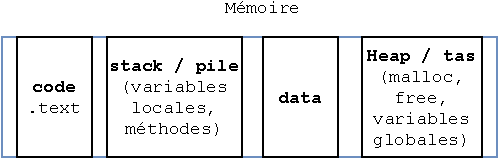
\includegraphics[scale=1,page=1]{Schemas-crop.pdf}
\end{center}
\paragraph{Éxecution sur le stack} : Ii le stack est éxécutable, il est possible d'y placer du code puis de l'éxécuter (ce qui est de moins en moins le cas).
\paragraph{ret2libc} : Permet de bypasser la non-éxécution du stack. Consiste à éxécuter du code dans une librairie comme libc.
\paragraph{ROP} : Return-Oriented Programming. Éxécution du programme lui-même pour effectuer l'attaque
\paragraph{ASLR} : Address Space Layout Randomization
\paragraph{PIE} : Position de l'éxécutable modifiée pour éviter qu'une attaque soit faite (ou la rendre plus difficile)





\end{document}